% !TeX document-id = {2dbf9b71-bbba-4dd9-bbd6-409e1a74ac36}
% !TeX TXS-program:compile = txs:///pdflatex/[--shell-escape] | txs:///biber | txs:///pdflatex/[--shell-escape]
\PassOptionsToPackage{svgnames}{xcolor}
\documentclass[spanish, utf8,handout]{beamer} % 
\usepackage[T1]{fontenc}
\usepackage[spanish]{babel}
\usepackage{amsmath,mathrsfs,amsfonts,amsthm}
\usepackage{tikz}
\usepackage{adjustbox}
\usepackage{caption}
\usepackage{pythontex}
%\usepackage[figurename=Figura]{caption}
\usepackage[backend=biber,style=numeric, defernumbers=true, sorting=ynt,maxbibnames=4,maxcitenames=4]{biblatex}
\addbibresource{bibliography/reference.bib}
%% Fix so biblatex works instead of natbib
\makeatletter
\let\c@author\relax
\makeatother
\let\bibhang\relax
\let\citename\relax
\let\bibfont\relax
\let\Citeauthor\relax
\expandafter\let\csname ver@natbib.sty\endcsname\relax

%% Fix headers and footers
\makeatletter
\def\ps@pprintTitle{%
	\let\@oddhead\@empty
	\let\@evenhead\@empty
	\def\@oddfoot{\centerline{\thepage}}%
	\let\@evenfoot\@oddfoot}
\makeatother

%% Load some packages and stuff
%\usepackage[backend=biber,style=numeric, defernumbers=true, sorting=ynt,maxbibnames=4,maxcitenames=4]{biblatex}
%% Library and stuff
\usepackage[style=numeric,sortcites=true,sorting=ynt,backend=biber]{biblatex}
%% biblatex med apa-style. Det vivill ha
\DeclareLanguageMapping{american}{american-apa} %% Vi vill ha svensk apa
\bibliography{../bibliography/reference}

\usepackage[T1]{fontenc}
\usepackage[spanish]{babel}
\usepackage{pifont}
\usepackage{geometry}
\usepackage[svgnames]{xcolor}
\usepackage{graphicx}
\usepackage{sagetex}
\usepackage{minted}
\usepackage{float}
\usepackage{tkz-graph}
\usepackage{txfonts}
\usepackage{amsmath,amsthm}
\theoremstyle{definition}
\usepackage{bm}
\usepackage[colorlinks=true,urlcolor=blue,linkcolor=black,anchorcolor=black,citecolor=black]{hyperref}
\hypersetup{pdfinfo={
		Title={El teorema de los cuatro colores},
		Author={Grupo Nº6},
		Keywords={teorema de los cuatro colores, cadena de Kempe, grafos planares, coloración de mapas},
		Subject={Introducción a la matemática discreta},
		Producer={TeXstudio 2.12.8},
		Creator={pdfTeX Version 3.14159265 TeX Live 2018 Debian}
}}


\usepackage{etoolbox}
\AtBeginDocument{%
	%\patchcmd{<cmd>}{<search>}{<replace>}{<success>}{<failure>}
	%\patchcmd{\ps@pprintTitle}% <cmd>
	%{Preprint submitted}% <search>
	%{To be submitted}% <replace>
	%{}{}% <succes><failure>
	\patchcmd{\MaketitleBox}{\vspace*{-20pt}\fi}{\fi}{}{}%
	\patchcmd{\abstract}{Abstract}{Resumen}{}{}
	\patchcmd{\keyword}{Keywords}{Palabras clave}{}{}
}

%\makeatletter
%\patchcmd{\ps@pprintTitle}{\footnotesize\itshape
%	Preprint submitted to \ifx\@journal\@empty Elsevier
%	\else\@journal\fi\hfill\today}{\relax}{}{}
%\makeatother

\makeatletter
\def\printFirstPageNotes{%
	\iflongmktitle
	\let\columnwidth=\textwidth\fi
	\ifx\@tnotes\@empty\else\@tnotes\fi
	\ifx\@nonumnotes\@empty\else\@nonumnotes\fi
	\ifx\@cornotes\@empty\else\@cornotes\fi
	\ifx\@elseads\@empty\relax\else
	\let\thefootnote\relax
	\footnotetext{\ifnum\theead=1\relax
		\textit{Correo electrónico:\space}\else
		\textit{Correos electrónicos:\space}\fi
		\@elseads}\fi
	\ifx\@elsuads\@empty\relax\else
	\let\thefootnote\relax
	\footnotetext{\textit{Sitio web:\space}%
		\@elsuads}\fi
	\ifx\@fnotes\@empty\else\@fnotes\fi
	\iflongmktitle\if@twocolumn
	\let\columnwidth=\Columnwidth\fi\fi
}
\makeatother

%% `Elsevier LaTeX' style
%\bibliographystyle{elsarticle-num}
\renewcommand{\spanishcontentsname}{Tabla de contenidos}
\renewcommand{\spanishfigurename}{Fig.}
\renewcommand{\listingscaption}{Programa}
%\newcommand{\MVAt}{{\usefont{U}{mvs}{m}{n}\symbol{`@}}}
\newtheorem{definition}{Definición}
\newtheorem{example}{Ejemplo}
\newtheorem{theorem}{Teorema}

\graphicspath{{../images/}}
\theoremstyle{definition}
\newtheorem{remark}{Observación}

\usetheme{CambridgeUS}
\usecolortheme{dolphin}
\useinnertheme{rectangles}
%\useoutertheme[hooks]{tree}

\usefonttheme[onlymath]{serif}

%\setbeamercovered{transparent}
\setbeamercovered{dynamic}

\setbeamertemplate{footline}[frame number]{}
\setbeamertemplate{navigation symbols}{}
\setbeamertemplate{footline}{}
\setbeamertemplate{headline}{}

\title[Teorema de los cuatro colores]{\Huge\sffamily El teorema de los cuatro colores}
\subtitle{Introducción a la matemática discreta CM -- 254}

\author[Grupo N$^\circ6$]{%
	\texorpdfstring{%
		\begin{columns}
			\column{.3\linewidth}
			\centering
			C. Aznarán Laos %\inst{1,2}
			\column{.3\linewidth}
			\centering
			F. Cruz Ordoñez %\inst{1,2}
		\end{columns}
		\vspace{12pt}
		\begin{columns}
			\column{.3\linewidth}
			\centering
			G. Quiroz Gómez %\inst{1,2}
			\column{.3\linewidth}
			\centering
			J. Navío Torres %\inst{1,2}
		\end{columns}
	}
	{Author 1, Author 2, Author 3}
}

\institute[FC -- UNI]{\large%\inst{1}
	Facultad de Ciencias \and%\inst{2}
	Universidad Nacional de Ingeniería
}
\date{18 de junio del 2018}

\graphicspath{{images/}}

\AtBeginSubsection[]
{
	\begin{frame}<beamer>
	\frametitle{\contentsname}
	\tableofcontents[
	currentsection,
	sectionstyle=show/show,
	subsectionstyle=show/shaded/hide%-show/shaded/hide
	]
\end{frame}
}

\begin{document}

\begin{frame}[plain]
\maketitle
\end{frame}

\begin{frame}{\contentsname}\transblindsvertical
\tableofcontents
\end{frame}

\section{Introducción}

\subsection{El problema de los cuatro colores}

\begin{frame}\transblindsvertical
\frametitle{\insertsubsection}

\begin{alertblock}{Pregunta} % 1852 Francis Guthrie
¿Es posible colorear cualquier mapa geográfico plano usando solamente \emph{\color{DarkBlue}cuatro colores}, de modo que dos países con frontera común tengan colores distintos? 
\end{alertblock}

\

\visible<2>{
\begin{minipage}[c]{6cm}
	\begin{figure}[H]
		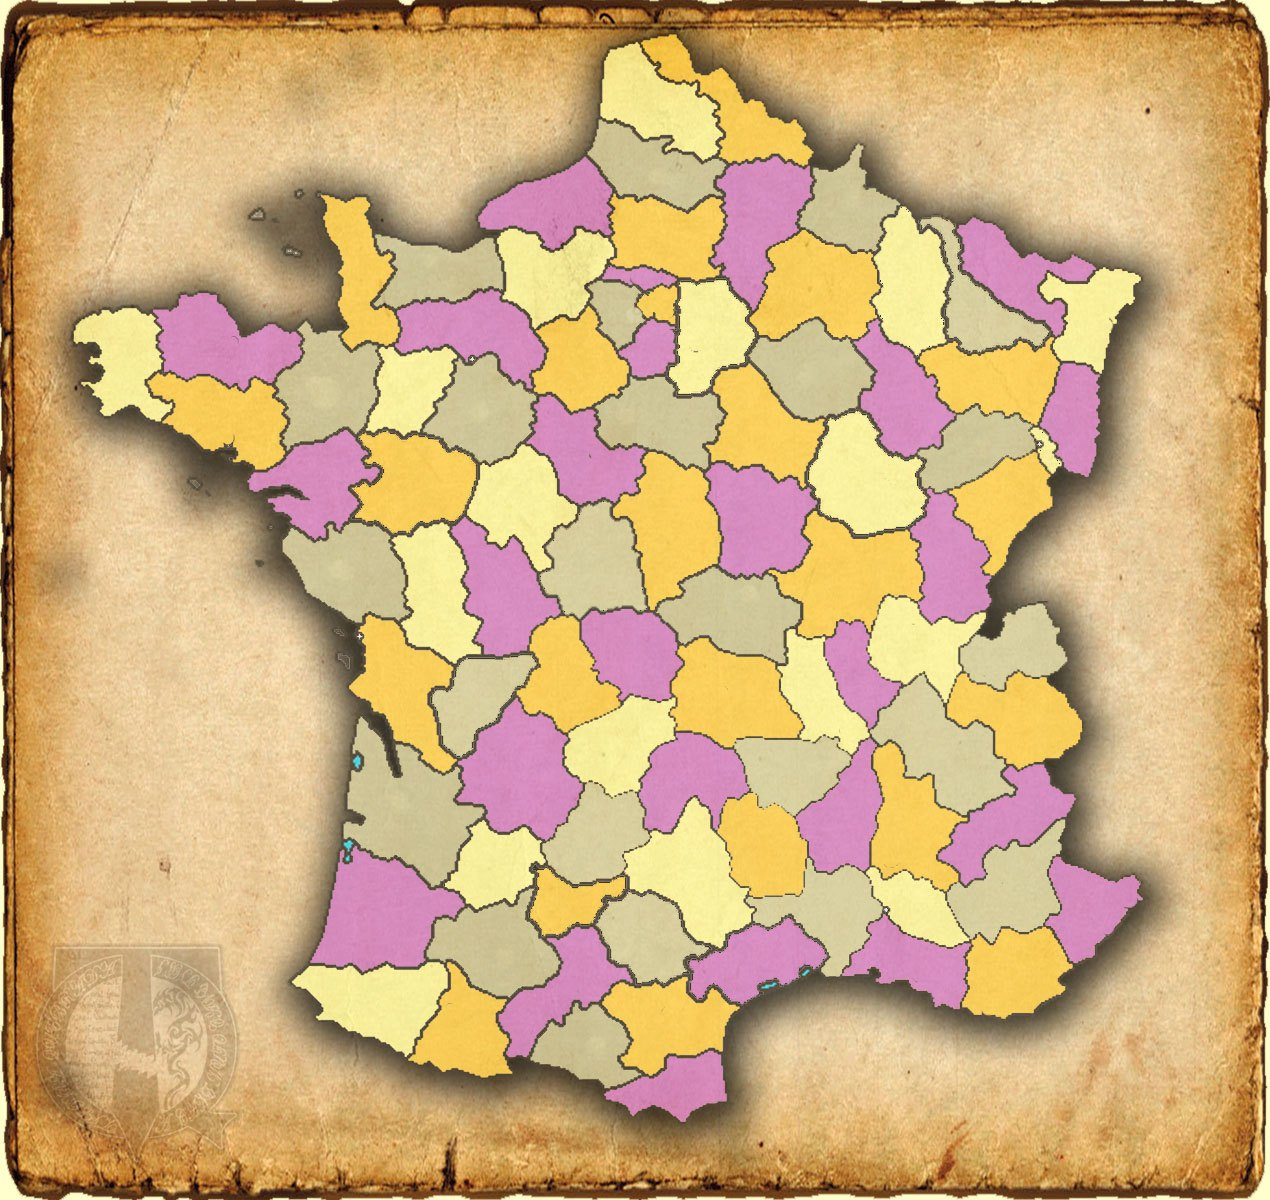
\includegraphics[width=4.2cm]{mapa-4-colores_HR.jpg}
		\caption{Mapa político coloreado}
	\end{figure}
\end{minipage}%\vspace{-1cm}
\begin{minipage}[c]{6cm}
	\begin{definition}[Mapa conexo]
	Un mapa es conexo\footnote{De una sola pieza.} y cada una \linebreak de sus regiones también es conexa.
	\end{definition}
\end{minipage}
}
\end{frame}

\begin{frame}{\insertsubsection}
\begin{remark}{}
Dos regiones {\color{red}no pueden tocarse solo en un punto}, y así, se pueden ignorar regiones con una única línea frontera.
\end{remark}

\visible<2>{
\begin{figure}[H]
	\centering
	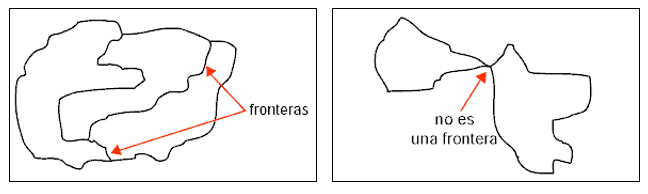
\includegraphics[height=3.3cm]{fronteras.png}
	\caption{Distinciones de frontera de un mapa.}
\end{figure}

Es un problema topológico: no importa la forma de las regiones, sino como están colocadas unas respecto a otras.
}
\end{frame}

{
	\usebackgroundtemplate{\centering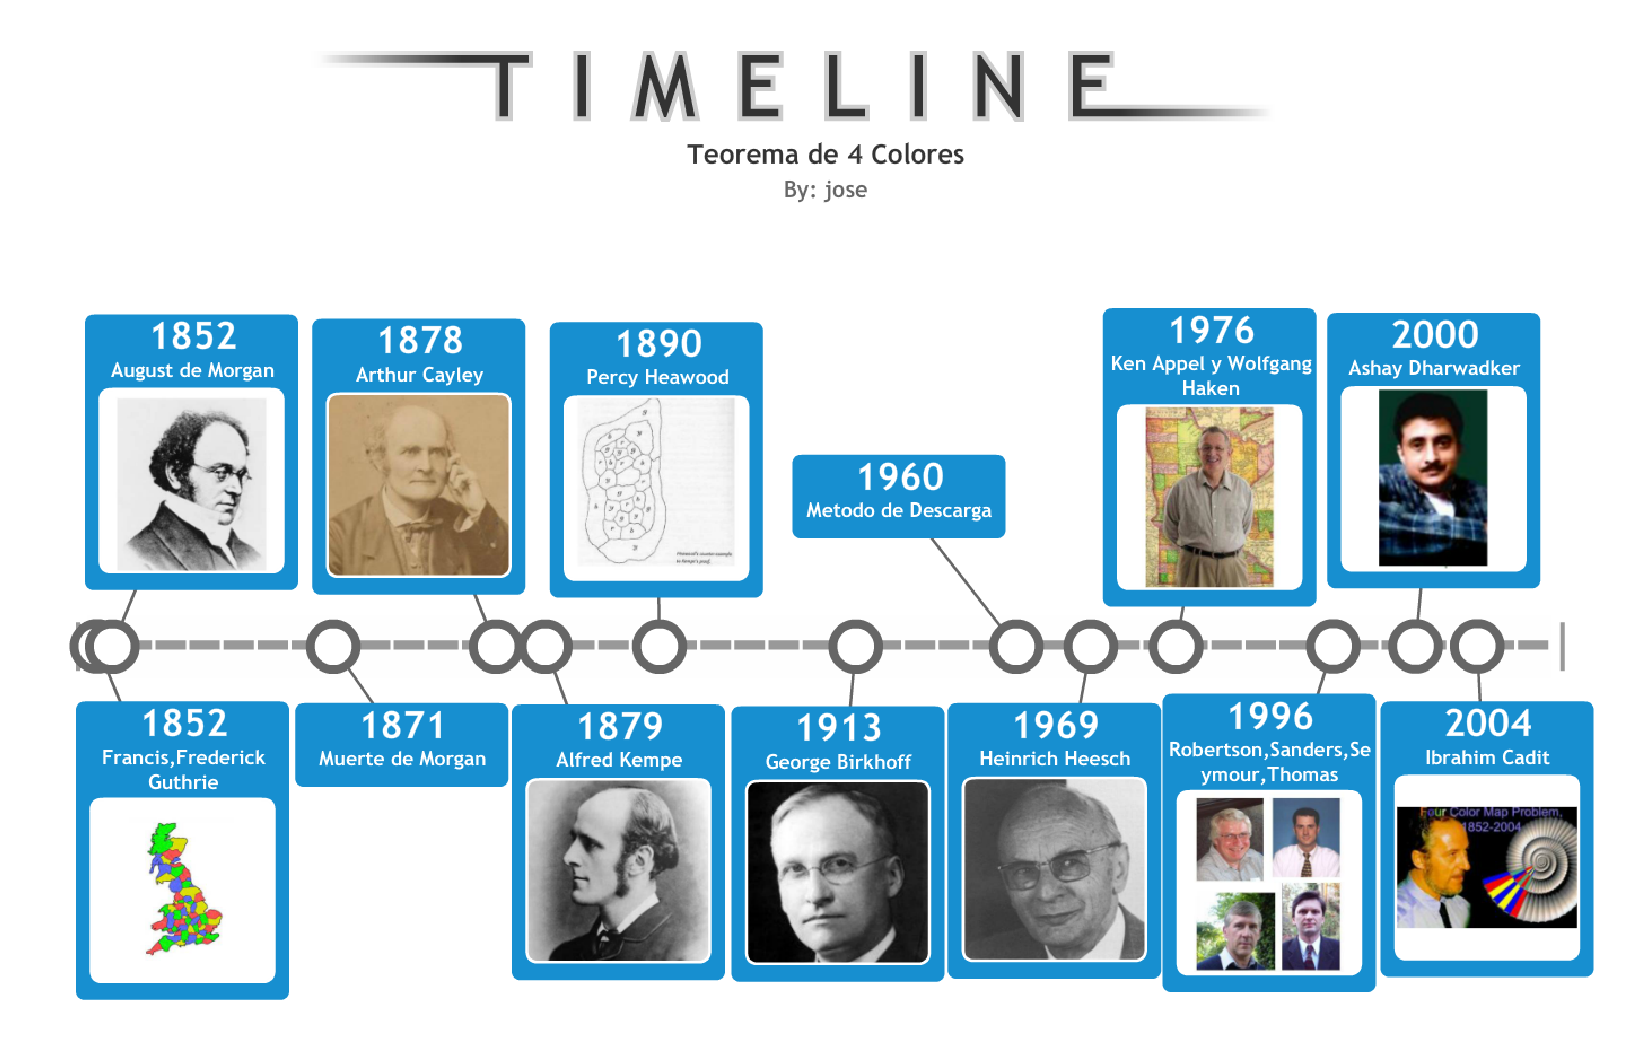
\includegraphics[width=\paperwidth]{crop}}
	\begin{frame}[plain]
\end{frame}
}

\subsection{Algunas fechas importantes}

\begin{frame}\transblindsvertical
\frametitle{\insertsubsection}

\begin{itemize}
	\item 1852: Francis Guthrie plantea el problema a su hermano Frederick y éste a Augustus de Morgan.
	
	\item  1878: Arthur Cayley publica el enunciado de la conjetura.
	
	\item  1879: Sir Alfred Bray Kempe publica su ``demostración''.
	
	\item  1913: George Birkhoff introduce la noción de configuración reducible.
	
	\item  1960: Se introduce el llamado método de descarga.
	
	\item  1969: Avances de Heinrich Heesch en reducibilidad y obtención de conjuntos inevitables de configuraciones.
	
	\item 1976: Ken Appel y Wolfgang Haken prueban con ayuda de un ordenador que sus 1.482 configuraciones son reducibles (50 días de cálculo).
	
	\item  1996: N. Robertson, D.P. Sanders, P. Seymour y R. Thomas mejoran la demostración con ayuda de ordenador (solo 633 configuraciones) y automatizan la prueba de la inevitabilidad.
\end{itemize}   
\end{frame}

\section{El ``camino'' hacia la demostración}

\subsection{La formulación de la conjetura}

\begin{frame}\transblindsvertical
\frametitle{\insertsubsection}

\begin{exampleblock}{Francis Guthrie (1839-1899)}
Abogado y botánico, observa que puede colorear un mapa complejo de los cantones de Inglaterra con 4 colores. En 1852, enuncia el problema a su hermano Frederick (University College London) y a éste a Augustus de Morgan. Francis Guthrie observa que 3 colores no son suficientes, con el diagrama crítico:
\end{exampleblock}
\visible<2>{
\begin{figure}[H]
\centering
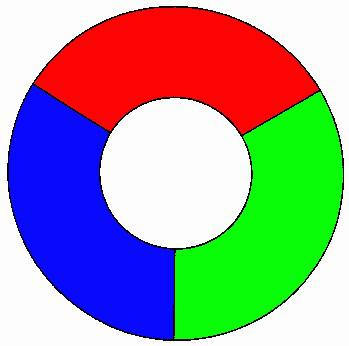
\includegraphics[scale=0.3]{diagrama.jpg}
\caption{Diagrama Crítico.}
\end{figure}
}
\end{frame}

\begin{frame}\transblindsvertical
\frametitle{\insertsection}

\begin{alertblock}{Difusión del teorema}
Augustus de Morgan (1806-1871) estaba muy interesado en la conjetura de los cuatro colores y lo difundió entre sus colegas. Una de las primeras personas con las que ``habló'' fue con el matemático y físico irlandés Sir William Rowan Hamilton (1805-1865), que no compartía el interés de De Morgan por el problema. Le escribe una carta el 23 de octubre de 1852.
\end{alertblock}

\visible<2>{
\begin{alertblock}{Respuesta de Hamilton}
Cuatro días después, Hamilton le contesta: ``I am not likely to attempt your ``quaternion'' of colours very soon''.
\end{alertblock}
} 
\end{frame}

\begin{frame}[allowframebreaks]
\frametitle{Definiciones previas}

\begin{definition}[Número cromático] 
Sea $G=(V,E)$ un grafo y sea $k$ un número natural. Una aplicación $c\colon V\to \{1,2,\ldots k\}$ se llama \emph{\color{DarkBlue}coloración del grafo} $G$ si $c(x)\neq c(y)$ se cumple para cada rama $\{x,y\}\in E$. \linebreak El \emph{\color{DarkBlue}número cromático} de $G$, denotado por $\chi(G)$, es el \emph{\color{red}mínimo valor} de $k$ para el cual existe una coloración $c\colon V(G)\to\{1,2\ldots,k\}$.
\end{definition}

\begin{definition}[Grafo Dual]
Sea $G=(V,E)$ un grafo planar con un dibujo planar fijo. Denotamos por $\mathcal{F}$ el conjunto de caras de $G$. Definimos un grafo, con posibles lazos y ramas múltiples, como $(\mathcal{F},E,\varepsilon)$, donde $\varepsilon$ se define como $\varepsilon(e)=\{F_i,F_j\}$ siempre que la rama $e$ sea una frontera común de las caras $F_i$ y $F_j$.

Este grafo $\left(\mathcal{F},E,\varepsilon\right)$ se le llama el dual de $G$ y se denota por $G^{\ast}$.	
\end{definition}


\begin{example}[Grafos Duales]
	Para construir una gráfica dual de un grafo plano $G$ se debe colocar un vértice dentro de cada región de $G$ e incluir la región infinita de $G$. Para cada arista compartida por las $2$ regiones, se debe dibujar una arista que conecte a los vértices dentro de estas regiones y para cada arista que se recorre $2$ veces en el camino cerrado alrededor de las aristas de una región se dibuja un lazo en el vértice de la región. 
\end{example}

\begin{figure}[H]
	\captionsetup{justification=centering,margin=0.5cm}
	\centering
	\begin{minipage}{.5\textwidth}
		\centering
		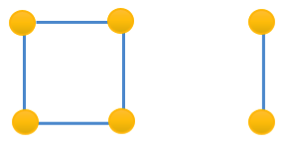
\includegraphics[width=3cm]{example1.png}
		\caption{Grafo $G$.}
	\end{minipage}%
	\begin{minipage}{0.5\textwidth}
		\centering
		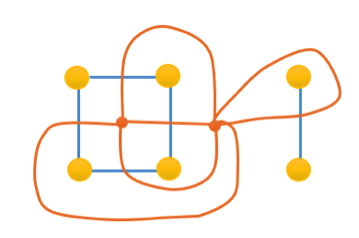
\includegraphics[width=3cm]{example2.png}
		\caption{Grafo $G$ y su dual $G^{\ast}$.}
	\end{minipage}
\end{figure}

\begin{example}[Grafos duales]
	Sea $G=(V,E)$ un grafo plano, se llama grafo dual de $G$ y se denota por $G^{\ast}$, aquel construido de la siguiente manera:
	
	\begin{enumerate}
		\item Se elige un punto $v_i$ en cada cara $F_i$ de $G$. Estos puntos son los vértices de $G^{\ast}$.
		
		\item Por cada arista $e\in E$ se traza una línea $e^{\ast}$ que atraviesa únicamente la arista $e$, y se unen los vértices $v_i$ pertenecientes a las caras adjuntas a $e$. Estas líneas son las aristas de $G^{\ast}$. A continuación se ilustra este procedimiento de construcción con un ejemplo:
	\end{enumerate}
\end{example}

\begin{figure}[H]
	\captionsetup{justification=centering,margin=0.5cm}
	\centering
	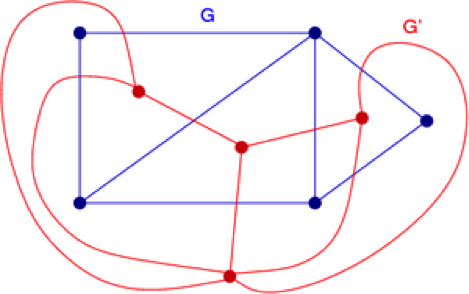
\includegraphics{example3.png}
	\caption{Grafo planar $G$ y	su grafo dual $G^{\prime}=G^{\ast}$.}
\end{figure}

\begin{definition}[Polinomio cromático]
Sea $G=(V,E)$ un grafo planar y $P(G,k)$ el número de vértices coloreados
El polinomio cromático cuenta el número de maneras que puede ser coloreado un grafo usando no más de número dado de colores.
\end{definition}

\begin{remark}
El polinomio cromático incluye al menos tanta información sobre la colorabilidad de G como el número cromático. De hecho, $\chi$ es el entero positivo más pequeño que no es una raíz del polinomio cromático

\begin{equation*}
\chi(G)=\min\{k\colon P(G,k)>0\}.
\end{equation*}
\end{remark}

\end{frame}

\subsection{La primera ``demostración'': las cadenas de \citeauthor{kempe}}

\begin{frame}\transblindsvertical
\frametitle{\insertsubsection}

Kempe se interesa por el problema de los cuatro colores tras la pregunta de Cayley en la London Mathematical Society.

\

\visible<2>{
En junio de 1879 obtiene su solución del teorema de los cuatro colores y lo publica en el Amer. Journal of Maths. En 1880, publica unas versiones. simplificadas de su prueba, donde corrige algunas erratas de su prueba original, pero deja intacto el error fatal.
}

\end{frame}

\begin{frame}
\frametitle{El algoritmo de las cadenas de Kempe}

\begin{definition}[Cadena de Kempe]
Sea $G$ un grafo planar cuyos vértices han sido coloreados apropiadamente y suponga $v\in V(G)$ es coloreado $C_1$. Definimos la \emph{cadena de Kempe} $C_1C_2$ que contiene a $v$ para ser el componente conexa maximal de $G$ que
\begin{enumerate}%[label=\arabic*]
	\item Contiene a $v$, y
	\item Contenga solo vértices que son coloreados con elementos desde $(C_1C_2)$.
\end{enumerate}
\end{definition}
\end{frame}

\subsection{Heawood y el error fatal de \citeauthor{kempe}}

\begin{frame}[allowframebreaks]
\frametitle{\insertsubsection}

\begin{example}[Grafo de Errera -- Contrajemplo]
Es un grafo planar de $17$ vértices y $45$ aristas que enreda las cadenas de Kempe en el algoritmo de Kempe y proporciona así un ejemplo de cómo falla la supuesta demostración de Kempe del teorema de cuatro colores.
\end{example}


\begin{remark}[Polinomio cromático del grafo de Errera]
A
\end{remark}
\end{frame}

\begin{frame}\transblindsvertical
\frametitle{\insertsubsection}

\begin{theorem}[Fórmula de Euler para mapas]
\begin{equation*}
\#\text{caras} - \#\text{aristas} + \#\text{vértices} = 2.	
\end{equation*}
\end{theorem}

\visible<2>{
\begin{figure}[H]
\centering
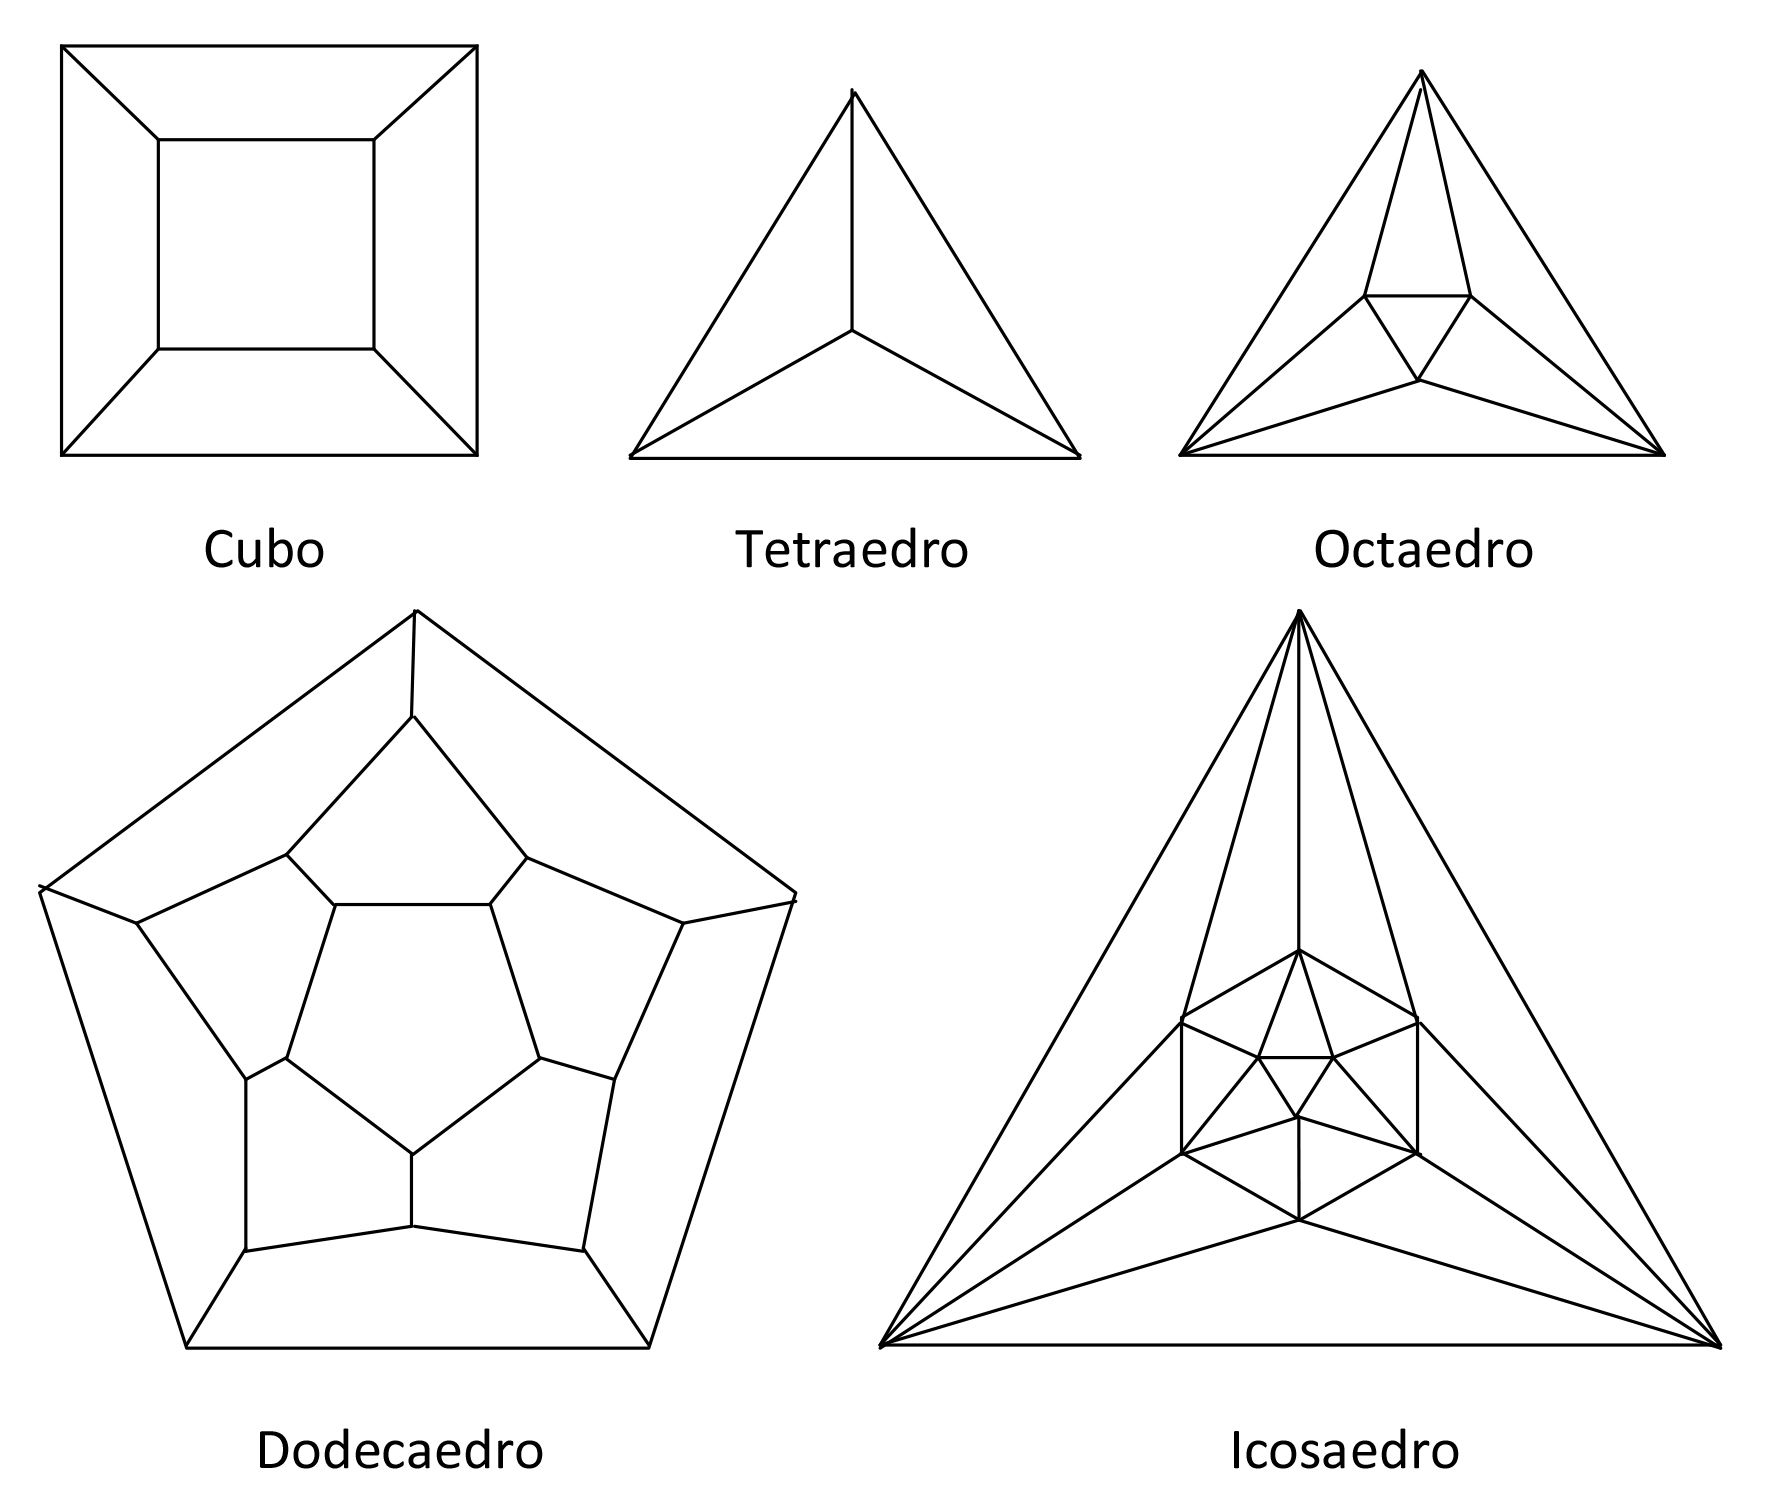
\includegraphics[height=5cm]{poliedros2.jpg}
\caption{Grafos de cada uno de los cinco sólidos platónicos.}
\end{figure}
}

\end{frame}

\subsection{Idea clave: la reducibilidad de mapas de \citeauthor{birkhoff}}

\begin{frame}
\frametitle{\insertsubsection}

\begin{theorem}[\citeauthor{birkhoff}]\normalfont
Solo una de las siguientes afirmaciones es verdadera:

\begin{enumerate}
	\item La conjetura de los cuatro colores puede ser falsa.
	
	\item Es posible hallar una colección finita de configuraciones reducibles \linebreak tal que cualquier mapa planar debe contener uno de ellos \linebreak (lo que probaría la conjetura de cuatro colores).
	
	\item La conjetura de cuatro colores puede ser cierta, pero pueden \linebreak requerirse métodos más complicados para una prueba.
\end{enumerate}
\end{theorem}
\end{frame}

\subsection{El método de descarga de \citeauthor{appel}}

\subsection{Una nueva demostración de \citeauthor{robertson}}

\section{Aplicaciones}

\subsection{El juego Hex}

\begin{frame}\transblindsvertical
\frametitle{\insertsubsection\footnote{Redescubierto en Priceton por John Nash en 1948.}}

\begin{columns}[t]
	\begin{column}{.4\textwidth}
			\begin{figure}[ht]
				%\centering
				\scalebox{.32}{% https://tex.stackexchange.com/questions/141911/drawing-hex-boards
\begin{tikzpicture}[rotate=90]
	%\showmynodenames%%<-- must precede the creation of the board if you want to see node names
	\drawhexboard{10}
	\draw[my hex path] ($(H1;1.corner 1)-(0,1cm)$) -- (H1;1.corner 1);
	\drawhexpath(1;1){1,2,3,4}
	\drawhexpath(2;2){6,5}
	\drawhexpath(3;2){1,2,3,4,5,6}
	\drawhexpath(3;1){2,1,6,5}
	\drawhexpath(4;1){1,2,3}
	\drawhexpath(5;2){1,2,3,4,5}
	
	\draw[my hex path] ($(H10;10.corner 3)+(1cm,0)$) -- (H10;10.corner 3);
	\drawhexpath(10;10){3,2,1,6,5}
	\drawhexpath(10;9){3,4}
	\drawhexpath(11;8){2,3,4}
	\drawhexpath(12;8){6,5,4,3,2}
\end{tikzpicture}}
				\caption{Patrón hexagonal.}
			\end{figure}%\adjincludegraphics[width=.8\linewidth,valign=t]{diagrama.jpg}
	\end{column}
	\begin{column}{.38\textwidth}
		\begin{flushleft}
		``El juego se basa en la simple propiedad geométrica de una superficie plana que dos líneas dentro de un cuadrado conectan cada una un par de lados opuestos deben cruzarse''.
		\end{flushleft}
		\		
		-- Piet Hein
	\end{column}
\end{columns}

\vspace*{5pt}

\begin{itemize}
	\item Reglas: Los jugadores se turnan para ocupar una celda y la otra para formar una cadena que conecta sus dos lados opuestos, y por lo tanto impide que la otra conecte sus lados, gana.
\end{itemize}
\end{frame}

%\begin{frame}\transblindsvertical
%\frametitle{\insertsubsection}
%\begin{tabular}{p{.3\textwidth} p{.7\textwidth}}
%	\adjincludegraphics[width=.8\linewidth,valign=t]{diagrama.jpg}
%	&
%	\raggedright\arraybackslash\textbf{``The problem of distinguishing prime numbers from composites, and of resolving composite numbers into their prime factors, is one of the most important and useful in all of arithmetic."}
%	
%	\hfill-- Carl Friedrich Gauss
%\end{tabular}
%
%\vspace*{10pt}
%
%\begin{itemize}
%	\item Pollard's $p-1$ algorithm (1974)
%	\vspace*{10pt}
%	\item Dixon's Random Squares Algorithm (1981)
%	\vspace*{10pt}
%	\item Quadratic Sieve (QS): Pomerance (1981)
%	\vspace*{10pt}
%	\item Williams' $p+1$ method (1982)
%\end{itemize}
%\end{frame}

\section{Conclusiones}

\subsection{Importancia del teorema para los matemáticos}

\begin{frame}
\frametitle{Agradecimientos}

\begin{center}\Large
	¡Muchas gracias!
\end{center}

Colaboradores:

\begin{enumerate}
	\item Elaboración de la línea de tiempo: José Navío.
	\item Tipografía en \LaTeX{}: Franss Cruz y Oromion.
	\item Explicación del contenido matemático: Gabriel Quiroz.
	\item Esquema de la exposición: MSc. Fidel Jara Huanca.
\end{enumerate}

\

{
\color{DarkBlue}
Presentación disponible en:
}
\begin{center}
\href{https://github.com/carlosal1015/4colores}{
\includegraphics[width=2.5cm]{Octocat.png}}
\end{center}
\hfill
\begin{flushright}
Dudas, sugerencias o preguntas a

\href{mailto:caznaranl@uni.pe}{caznaranl\MVAt uni.pe}
\end{flushright}
\end{frame}

\begin{frame}[allowframebreaks]\transblindsvertical
\frametitle{Referencias}

\begin{itemize}
	\item Libros
	\nocite{*}
	\printbibliography[heading=none,keyword=book]
	
	\item Artículos matemáticos
	\printbibliography[heading=none,keyword=paper]
	
	\item Sitios web
	\printbibliography[heading=none,keyword=online]
\end{itemize}
\end{frame}

\end{document}